% Options for packages loaded elsewhere
% Options for packages loaded elsewhere
\PassOptionsToPackage{unicode}{hyperref}
\PassOptionsToPackage{hyphens}{url}
\PassOptionsToPackage{dvipsnames,svgnames,x11names}{xcolor}
%
\documentclass[
  letterpaper,
  DIV=11,
  numbers=noendperiod]{scrreprt}
\usepackage{xcolor}
\usepackage{amsmath,amssymb}
\setcounter{secnumdepth}{5}
\usepackage{iftex}
\ifPDFTeX
  \usepackage[T1]{fontenc}
  \usepackage[utf8]{inputenc}
  \usepackage{textcomp} % provide euro and other symbols
\else % if luatex or xetex
  \usepackage{unicode-math} % this also loads fontspec
  \defaultfontfeatures{Scale=MatchLowercase}
  \defaultfontfeatures[\rmfamily]{Ligatures=TeX,Scale=1}
\fi
\usepackage{lmodern}
\ifPDFTeX\else
  % xetex/luatex font selection
\fi
% Use upquote if available, for straight quotes in verbatim environments
\IfFileExists{upquote.sty}{\usepackage{upquote}}{}
\IfFileExists{microtype.sty}{% use microtype if available
  \usepackage[]{microtype}
  \UseMicrotypeSet[protrusion]{basicmath} % disable protrusion for tt fonts
}{}
\makeatletter
\@ifundefined{KOMAClassName}{% if non-KOMA class
  \IfFileExists{parskip.sty}{%
    \usepackage{parskip}
  }{% else
    \setlength{\parindent}{0pt}
    \setlength{\parskip}{6pt plus 2pt minus 1pt}}
}{% if KOMA class
  \KOMAoptions{parskip=half}}
\makeatother
% Make \paragraph and \subparagraph free-standing
\makeatletter
\ifx\paragraph\undefined\else
  \let\oldparagraph\paragraph
  \renewcommand{\paragraph}{
    \@ifstar
      \xxxParagraphStar
      \xxxParagraphNoStar
  }
  \newcommand{\xxxParagraphStar}[1]{\oldparagraph*{#1}\mbox{}}
  \newcommand{\xxxParagraphNoStar}[1]{\oldparagraph{#1}\mbox{}}
\fi
\ifx\subparagraph\undefined\else
  \let\oldsubparagraph\subparagraph
  \renewcommand{\subparagraph}{
    \@ifstar
      \xxxSubParagraphStar
      \xxxSubParagraphNoStar
  }
  \newcommand{\xxxSubParagraphStar}[1]{\oldsubparagraph*{#1}\mbox{}}
  \newcommand{\xxxSubParagraphNoStar}[1]{\oldsubparagraph{#1}\mbox{}}
\fi
\makeatother

\usepackage{color}
\usepackage{fancyvrb}
\newcommand{\VerbBar}{|}
\newcommand{\VERB}{\Verb[commandchars=\\\{\}]}
\DefineVerbatimEnvironment{Highlighting}{Verbatim}{commandchars=\\\{\}}
% Add ',fontsize=\small' for more characters per line
\usepackage{framed}
\definecolor{shadecolor}{RGB}{241,243,245}
\newenvironment{Shaded}{\begin{snugshade}}{\end{snugshade}}
\newcommand{\AlertTok}[1]{\textcolor[rgb]{0.68,0.00,0.00}{#1}}
\newcommand{\AnnotationTok}[1]{\textcolor[rgb]{0.37,0.37,0.37}{#1}}
\newcommand{\AttributeTok}[1]{\textcolor[rgb]{0.40,0.45,0.13}{#1}}
\newcommand{\BaseNTok}[1]{\textcolor[rgb]{0.68,0.00,0.00}{#1}}
\newcommand{\BuiltInTok}[1]{\textcolor[rgb]{0.00,0.23,0.31}{#1}}
\newcommand{\CharTok}[1]{\textcolor[rgb]{0.13,0.47,0.30}{#1}}
\newcommand{\CommentTok}[1]{\textcolor[rgb]{0.37,0.37,0.37}{#1}}
\newcommand{\CommentVarTok}[1]{\textcolor[rgb]{0.37,0.37,0.37}{\textit{#1}}}
\newcommand{\ConstantTok}[1]{\textcolor[rgb]{0.56,0.35,0.01}{#1}}
\newcommand{\ControlFlowTok}[1]{\textcolor[rgb]{0.00,0.23,0.31}{\textbf{#1}}}
\newcommand{\DataTypeTok}[1]{\textcolor[rgb]{0.68,0.00,0.00}{#1}}
\newcommand{\DecValTok}[1]{\textcolor[rgb]{0.68,0.00,0.00}{#1}}
\newcommand{\DocumentationTok}[1]{\textcolor[rgb]{0.37,0.37,0.37}{\textit{#1}}}
\newcommand{\ErrorTok}[1]{\textcolor[rgb]{0.68,0.00,0.00}{#1}}
\newcommand{\ExtensionTok}[1]{\textcolor[rgb]{0.00,0.23,0.31}{#1}}
\newcommand{\FloatTok}[1]{\textcolor[rgb]{0.68,0.00,0.00}{#1}}
\newcommand{\FunctionTok}[1]{\textcolor[rgb]{0.28,0.35,0.67}{#1}}
\newcommand{\ImportTok}[1]{\textcolor[rgb]{0.00,0.46,0.62}{#1}}
\newcommand{\InformationTok}[1]{\textcolor[rgb]{0.37,0.37,0.37}{#1}}
\newcommand{\KeywordTok}[1]{\textcolor[rgb]{0.00,0.23,0.31}{\textbf{#1}}}
\newcommand{\NormalTok}[1]{\textcolor[rgb]{0.00,0.23,0.31}{#1}}
\newcommand{\OperatorTok}[1]{\textcolor[rgb]{0.37,0.37,0.37}{#1}}
\newcommand{\OtherTok}[1]{\textcolor[rgb]{0.00,0.23,0.31}{#1}}
\newcommand{\PreprocessorTok}[1]{\textcolor[rgb]{0.68,0.00,0.00}{#1}}
\newcommand{\RegionMarkerTok}[1]{\textcolor[rgb]{0.00,0.23,0.31}{#1}}
\newcommand{\SpecialCharTok}[1]{\textcolor[rgb]{0.37,0.37,0.37}{#1}}
\newcommand{\SpecialStringTok}[1]{\textcolor[rgb]{0.13,0.47,0.30}{#1}}
\newcommand{\StringTok}[1]{\textcolor[rgb]{0.13,0.47,0.30}{#1}}
\newcommand{\VariableTok}[1]{\textcolor[rgb]{0.07,0.07,0.07}{#1}}
\newcommand{\VerbatimStringTok}[1]{\textcolor[rgb]{0.13,0.47,0.30}{#1}}
\newcommand{\WarningTok}[1]{\textcolor[rgb]{0.37,0.37,0.37}{\textit{#1}}}

\usepackage{longtable,booktabs,array}
\usepackage{calc} % for calculating minipage widths
% Correct order of tables after \paragraph or \subparagraph
\usepackage{etoolbox}
\makeatletter
\patchcmd\longtable{\par}{\if@noskipsec\mbox{}\fi\par}{}{}
\makeatother
% Allow footnotes in longtable head/foot
\IfFileExists{footnotehyper.sty}{\usepackage{footnotehyper}}{\usepackage{footnote}}
\makesavenoteenv{longtable}
\usepackage{graphicx}
\makeatletter
\newsavebox\pandoc@box
\newcommand*\pandocbounded[1]{% scales image to fit in text height/width
  \sbox\pandoc@box{#1}%
  \Gscale@div\@tempa{\textheight}{\dimexpr\ht\pandoc@box+\dp\pandoc@box\relax}%
  \Gscale@div\@tempb{\linewidth}{\wd\pandoc@box}%
  \ifdim\@tempb\p@<\@tempa\p@\let\@tempa\@tempb\fi% select the smaller of both
  \ifdim\@tempa\p@<\p@\scalebox{\@tempa}{\usebox\pandoc@box}%
  \else\usebox{\pandoc@box}%
  \fi%
}
% Set default figure placement to htbp
\def\fps@figure{htbp}
\makeatother


% definitions for citeproc citations
\NewDocumentCommand\citeproctext{}{}
\NewDocumentCommand\citeproc{mm}{%
  \begingroup\def\citeproctext{#2}\cite{#1}\endgroup}
\makeatletter
 % allow citations to break across lines
 \let\@cite@ofmt\@firstofone
 % avoid brackets around text for \cite:
 \def\@biblabel#1{}
 \def\@cite#1#2{{#1\if@tempswa , #2\fi}}
\makeatother
\newlength{\cslhangindent}
\setlength{\cslhangindent}{1.5em}
\newlength{\csllabelwidth}
\setlength{\csllabelwidth}{3em}
\newenvironment{CSLReferences}[2] % #1 hanging-indent, #2 entry-spacing
 {\begin{list}{}{%
  \setlength{\itemindent}{0pt}
  \setlength{\leftmargin}{0pt}
  \setlength{\parsep}{0pt}
  % turn on hanging indent if param 1 is 1
  \ifodd #1
   \setlength{\leftmargin}{\cslhangindent}
   \setlength{\itemindent}{-1\cslhangindent}
  \fi
  % set entry spacing
  \setlength{\itemsep}{#2\baselineskip}}}
 {\end{list}}
\usepackage{calc}
\newcommand{\CSLBlock}[1]{\hfill\break\parbox[t]{\linewidth}{\strut\ignorespaces#1\strut}}
\newcommand{\CSLLeftMargin}[1]{\parbox[t]{\csllabelwidth}{\strut#1\strut}}
\newcommand{\CSLRightInline}[1]{\parbox[t]{\linewidth - \csllabelwidth}{\strut#1\strut}}
\newcommand{\CSLIndent}[1]{\hspace{\cslhangindent}#1}



\setlength{\emergencystretch}{3em} % prevent overfull lines

\providecommand{\tightlist}{%
  \setlength{\itemsep}{0pt}\setlength{\parskip}{0pt}}



 


\usepackage{makeidx}
\makeindex
\KOMAoption{captions}{tableheading}
\makeatletter
\@ifpackageloaded{bookmark}{}{\usepackage{bookmark}}
\makeatother
\makeatletter
\@ifpackageloaded{caption}{}{\usepackage{caption}}
\AtBeginDocument{%
\ifdefined\contentsname
  \renewcommand*\contentsname{Table of contents}
\else
  \newcommand\contentsname{Table of contents}
\fi
\ifdefined\listfigurename
  \renewcommand*\listfigurename{List of Figures}
\else
  \newcommand\listfigurename{List of Figures}
\fi
\ifdefined\listtablename
  \renewcommand*\listtablename{List of Tables}
\else
  \newcommand\listtablename{List of Tables}
\fi
\ifdefined\figurename
  \renewcommand*\figurename{Figure}
\else
  \newcommand\figurename{Figure}
\fi
\ifdefined\tablename
  \renewcommand*\tablename{Table}
\else
  \newcommand\tablename{Table}
\fi
}
\@ifpackageloaded{float}{}{\usepackage{float}}
\floatstyle{ruled}
\@ifundefined{c@chapter}{\newfloat{codelisting}{h}{lop}}{\newfloat{codelisting}{h}{lop}[chapter]}
\floatname{codelisting}{Listing}
\newcommand*\listoflistings{\listof{codelisting}{List of Listings}}
\makeatother
\makeatletter
\makeatother
\makeatletter
\@ifpackageloaded{caption}{}{\usepackage{caption}}
\@ifpackageloaded{subcaption}{}{\usepackage{subcaption}}
\makeatother
\usepackage{bookmark}
\IfFileExists{xurl.sty}{\usepackage{xurl}}{} % add URL line breaks if available
\urlstyle{same}
\hypersetup{
  pdftitle={IDEA Growth Scorecard Documentation},
  pdfauthor={Hilary Doe},
  colorlinks=true,
  linkcolor={blue},
  filecolor={Maroon},
  citecolor={Blue},
  urlcolor={Blue},
  pdfcreator={LaTeX via pandoc}}


\title{IDEA Growth Scorecard Documentation}
\author{Hilary Doe}
\date{2025-09-11}
\begin{document}
\maketitle

\renewcommand*\contentsname{Table of contents}
{
\hypersetup{linkcolor=}
\setcounter{tocdepth}{2}
\tableofcontents
}

\bookmarksetup{startatroot}

\chapter*{Introduction / Index}\label{introduction-index}
\addcontentsline{toc}{chapter}{Introduction / Index}

\markboth{Introduction / Index}{Introduction / Index}

\section*{Purpose}\label{purpose}
\addcontentsline{toc}{section}{Purpose}

\markright{Purpose}

The Growth Scorecards were designed for use by IDEA's Growth team to
provide relevant data and insights to guide strategic decision making as
IDEA Texas considers expansion, consolidation, and/or closure of schools
and regions. Currently, the Growth Scorecards include only data from
IDEA's Texas regions.

Although our goal is to establish a single source of relevant data, such
as school performance, enrollment, and financial characteristics, not
all desired data can easily be pulled and cleaned within R without
reaching out to partners within IDEA.

The purpose of this resource is to document where each metric comes
from, how it is defined, and how to reproduce calculations for future
iterations.

\section*{Structure}\label{structure}
\addcontentsline{toc}{section}{Structure}

\markright{Structure}

Each chapter of this resource will contain information about a related
section of metrics:

\begin{itemize}
\tightlist
\item
  Chapter~\ref{sec-Performance}

  \begin{itemize}
  \tightlist
  \item
    Section~\ref{sec-Account}
  \item
    Section~\ref{sec-STAAR}
  \item
    Section~\ref{sec-Fail}
  \end{itemize}
\item
  Chapter~\ref{sec-Finance}

  \begin{itemize}
  \tightlist
  \item
    Section~\ref{sec-DaysCash}
  \item
    Section~\ref{sec-DebtRatio}
  \item
    Section~\ref{sec-PerPupil}
  \end{itemize}
\item
  Chapter~\ref{sec-Capital}

  \begin{itemize}
  \tightlist
  \item
    Section~\ref{sec-DebtCov}
  \end{itemize}
\item
  Chapter~\ref{sec-TeacherSupply}

  \begin{itemize}
  \tightlist
  \item
    Section~\ref{sec-TeachHire}
  \item
    Section~\ref{sec-YOYTeach}
  \end{itemize}
\item
  Chapter~\ref{sec-05HQBand}

  \begin{itemize}
  \tightlist
  \item
    Section~\ref{sec-05Leaders}
  \item
    Section~\ref{sec-05APIVacancy}
  \item
    Section~\ref{sec-05CAPGrads}
  \end{itemize}
\item
  Chapter~\ref{sec-06Enroll}

  \begin{itemize}
  \tightlist
  \item
    Section~\ref{sec-06Goal}
  \item
    Section~\ref{sec-06Cap}
  \item
    Section~\ref{sec-06Persist}
  \end{itemize}
\end{itemize}

\bookmarksetup{startatroot}

\chapter{School Performance Data}\label{sec-Performance}

\section{Meets STAAR Performance Standards for Math and
ELA}\label{sec-STAAR}

The State of Texas Assessments of Academic Readiness (STAAR) assessments
are Texas' annual standardized tests. For the Growth Scorecards, we are
using results of all math and English Language Arts (ELA) standard
assessments including the STAAR assessments of Reading and Math
conducted in grades 3-8 and End-of-Course (EOC) assessments of Algebra
I, English I, and English II.

\begin{quote}
``All STAAR assessments, excluding STAAR Alt 2, have three performance
standards: Approaches, Meets, and Masters {[}\ldots{]} These three
performance levels are NOT mutually exclusive, meaning that students
that achieve the Masters standard are included in the Meets count and
the Approaches count, and students achieving the Meets standard are
included in the Approaches count.'' (IDEA RAP Team, n.d.)
\end{quote}

Percentage of students Meeting performance standards for Math and ELA
are calculated at the entity, region, and campus level as:

\[\% \text{ Meeting Standards} = \frac{\# \text{ of Students Meeting in Subject}}{\# \text{ of Students with Scored STAAR or EOC for Subject}}*100\]

\subsection{Notes \& Exclusions}\label{notes-exclusions}

\begin{itemize}
\item
  Students may retake a STAAR assessment more than once within the same
  academic year. For students that had more than one score for the same
  assessment and academic year, we use the highest-scoring test. Meaning
  that if they scored in the ``Approaches'' range at one point and
  scored in the ``Meets'' range at another point, they are counted as
  ``Meeting'' the performance standards for that subject.
\item
  This metric does not include STAAR Alternate 2 tests, which are
  typically given to students with significant cognitive disabilities,
  and for which the typical three-level performance standards to not
  apply.
\item
  The data warehouse does not include any STAAR or EOC assessments for
  students above 5th grade at the Travis campus in Midland ISD (Travis
  Academy students are included).

  \begin{itemize}
  \tightlist
  \item
    IDEA Travis is a unique partnership between Midland ISD and IDEA
    Public schools, where the data is technically owned by Midland ISD
    and shared with IDEA.
  \end{itemize}
\end{itemize}

\subsection{Source}\label{source}

The STAAR data includes STAAR and high school level End-of-Course (EOC)
assessments stored in IDEA's data warehouse(IDEA Public Schools Data
Warehouse 2025b).

\begin{Shaded}
\begin{Highlighting}[]
\NormalTok{STAAR }\OtherTok{\textless{}{-}} \FunctionTok{get\_table}\NormalTok{(}\AttributeTok{.table\_name =} \StringTok{"STAAR"}\NormalTok{, }
                   \AttributeTok{.database\_name =} \StringTok{"Dashboard"}\NormalTok{,}
                   \AttributeTok{.schema =} \StringTok{"dbo"}\NormalTok{, }
                   \AttributeTok{.server\_name =} \StringTok{"RGVPDRA{-}DASQL"}
\NormalTok{                  ) }\SpecialCharTok{\%\textgreater{}\%}
  \FunctionTok{filter}\NormalTok{(}
    \DocumentationTok{\#\# Includes STAAR but not STAAR Alt 2 }
\NormalTok{      TestVersion }\SpecialCharTok{==} \StringTok{"S"}\NormalTok{, }
    \DocumentationTok{\#\# Includes Scored assessments only}
\NormalTok{      ScoreCode }\SpecialCharTok{==} \StringTok{"S"}\NormalTok{, }
    \DocumentationTok{\#\# Includes Math and English }
\NormalTok{    (SubjectCode }\SpecialCharTok{==} \StringTok{"Math"} \SpecialCharTok{|}
\NormalTok{     SubjectCode }\SpecialCharTok{==} \StringTok{"Reading"} \SpecialCharTok{|}
\NormalTok{     SubjectCode }\SpecialCharTok{==} \StringTok{"Algebra I"} \SpecialCharTok{|}
\NormalTok{     SubjectCode }\SpecialCharTok{==} \StringTok{"English I"} \SpecialCharTok{|}
\NormalTok{     SubjectCode }\SpecialCharTok{==} \StringTok{"English II"}\NormalTok{),}
    \DocumentationTok{\#\# Select desired school years}
\NormalTok{    (SchoolYear }\SpecialCharTok{==} \StringTok{"2024{-}2025"} \SpecialCharTok{|}
\NormalTok{     SchoolYear }\SpecialCharTok{==} \StringTok{"2023{-}2024"}\NormalTok{)}
\NormalTok{  )}
\end{Highlighting}
\end{Shaded}

\section{Accountability Ratings}\label{sec-Account}

Texas Education Agency (TEA) uses the an accountability rating system to
evaluate the academic performance of all Texas public districts,
including public school districts and open-enrollment charter schools
(Texas Education Agency 2025b). Annual ratings are based on three
domains:

\begin{enumerate}
\def\labelenumi{\arabic{enumi}.}
\tightlist
\item
  Student Achievement (STAAR, EOC, College, Career, and Military
  Readiness, graduation rates)
\item
  School Progress (student academic growth, achievement relative to
  schools with similar economic disadvantage levels)
\item
  Closing the Gaps (progress among students from specific groups,
  e.g.~racial/ethnic groups, special education, Emergent Bilingual or
  English learner, etc.)
\end{enumerate}

Each district and campus receives an A-F letter grade for each of the
three domains and one overall score with associated letter grade. For
more information on how specific ratings are calculated by TEA, find the
most recent Accountability Rating System manual (Texas Education Agency
2025b).

\subsection{Percentage of Schools Rated A \& B and D \&
F}\label{percentage-of-schools-rated-a-b-and-d-f}

For the percentage of schools with specific letter grade accountability
ratings, each individual school (Academy, College Prep) has its own
rating. The metrics are calculated at the entity and region level as
follows:
\[{\% \text{ of Schools Rated A or B}} = \frac{(\# \text{ of Schools Rated A}) + (\# \text{ of Schools Rated B})}{\text{Total } \# \text{ of Schools with Rating in Region}}*100\]
\[{\% \text{ of Schools Rated D or F}} = \frac{(\# \text{ of Schools Rated D}) + (\# \text{ of Schools Rated F})}{\text{Total } \# \text{ of Schools with Rating in Region}}*100\]

\subsection{Multi-Year Failure}\label{sec-Fail}

For the multi-year failure metric, we considered schools with an overall
rating \textless70 to be ``failing'' and any schools with a failing
rating for two subsequent rated years to have experienced a multi-year
failure. To be counted as being in multi-year failure for the 2024-2025
school year, a school must have an overall rating score of \textless70
in the 2024-2025 school year and the 2023-2024 school year.

We calculated the number and percentage of schools in each region
multi-year filaure for the 2024-2025 year.

\[{\% \text{ of Schools with Multi-Year Failure}} = \frac{\# \text{ of Schools with Multi-Year Failure}}{\text{Total } \# \text{ of Schools with Rating in Region}}*100\]

Individual schools are marked has having a previous had multi-year
failure if the school had a rating \textless70 for any two or more
subsequently rated years prior to 2024-2025.

\subsubsection{Notes \& Exclusions}\label{notes-exclusions-1}

\begin{itemize}
\tightlist
\item
  No schools received ratings for the 2019-2020 and 2020-2021 school
  years, because of the COVID-19 pandemic. This metric considers a
  school to have a multi-year failure if they were below the threshold
  in 2018-2019 and 2021-2022, because they were below the threshold for
  two subsequently rated years.
\end{itemize}

\subsection{Source}\label{source-1}

For the each of the school years, accountability ratings were downloaded
from the
\href{https://rptsvr1.tea.texas.gov/perfreport/account/index.html}{TEA
Accountability Ratings} page, by selecting the appropriate year and
navigating to the relevant Data Download page.

Although the download page structure differs some by year, in each case
parameters were set to campus-level report, selecting the accountability
summary (Texas Education Agency 2018, 2019, 2022, 2023, 2024, 2025a), as
seen in the screenshots below.

\begin{figure}[H]

{\centering 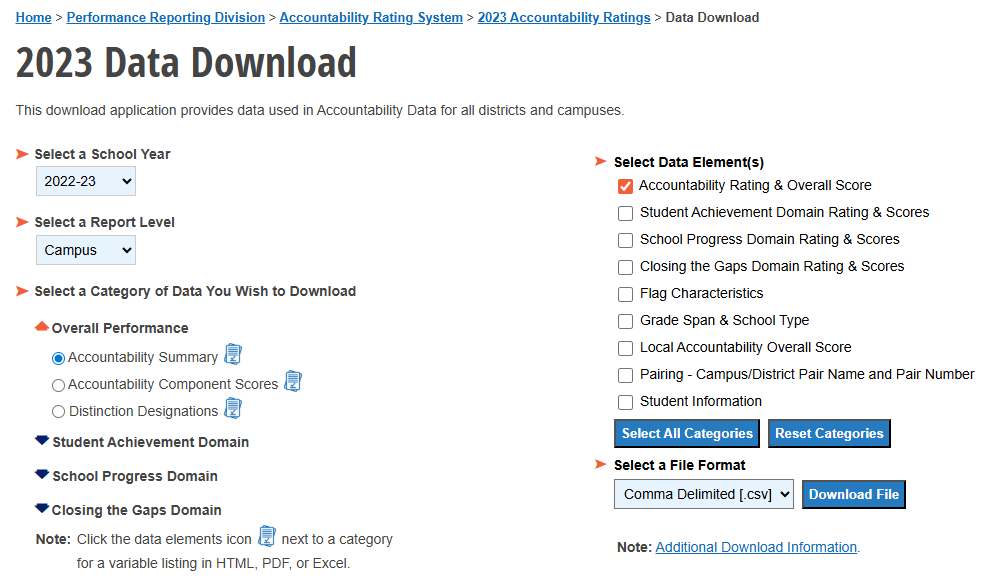
\includegraphics[width=6.25in,height=\textheight,keepaspectratio]{visuals/2023_accountability_screenshot.png}

}

\caption{Screenshot of download parameters for 2022-2023 accountability
ratings}

\end{figure}%

For 2022-2023 through 2024-2025, we requested the Accountability Rating
and Overall Score data elements, but such download options were not
available for the earlier years.

\begin{figure}[H]

{\centering 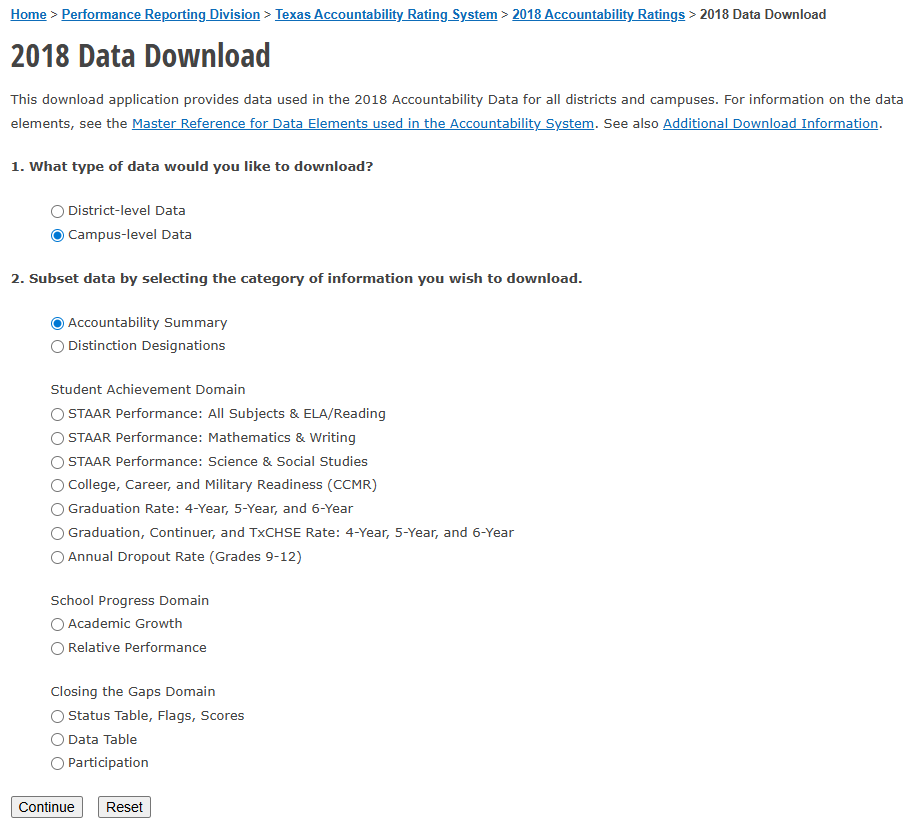
\includegraphics[width=6.25in,height=\textheight,keepaspectratio]{visuals/2018_accountability_screenshot.png}

}

\caption{Screenshot of download parameters for 2017-2018 accountability
ratings.}

\end{figure}%

Although the script to call each year varies slightly, each includes a
filter to maintain all IDEA TX schools, include any ratings of IDEA
Travis schools that are a partnership with Midland ISD. At this time,
IDEA Travis schools are considered one school, as ``IDEA Travis
Academy,'' by TEA. If in the future, IDEA Travis schools are separated
with TEA records, the filter shown below should hopefully help to
retrieve any IDEA Travis schools when applied to the appropriate year.

\begin{Shaded}
\begin{Highlighting}[]
\NormalTok{ratings\_25  }\OtherTok{\textless{}{-}} \FunctionTok{read.csv}\NormalTok{(}
  \StringTok{"filepath/2025\_Campus\_Accountability\_Summary.csv"}\NormalTok{, }
    \AttributeTok{header =} \ConstantTok{TRUE}\NormalTok{, }
    \AttributeTok{as.is =} \FunctionTok{c}\NormalTok{(}\StringTok{"CAMPUS"}\NormalTok{, }\StringTok{"DISTRICT"}\NormalTok{, }\StringTok{"COUNTY"}\NormalTok{, }\StringTok{"REGION"}\NormalTok{),}
    \AttributeTok{colClasses =} \StringTok{"character"}
\NormalTok{  ) }\SpecialCharTok{\%\textgreater{}\%}
  \FunctionTok{filter}\NormalTok{( }\CommentTok{\# Keeps IDEA TX and the Travis Midland schools}
\NormalTok{    DISTRICT }\SpecialCharTok{==} \StringTok{"108807"} \SpecialCharTok{|} 
\NormalTok{    CAMPUS }\SpecialCharTok{==} \StringTok{"165901139"} \SpecialCharTok{|} 
\NormalTok{    CAMPUS }\SpecialCharTok{==} \StringTok{"165901138"} \SpecialCharTok{|} 
\NormalTok{    CAMPUS }\SpecialCharTok{==} \StringTok{"165901137"}\NormalTok{ ) }\SpecialCharTok{\%\textgreater{}\%} 
  \FunctionTok{select}\NormalTok{(CAMPUS, CAMPNAME, DISTRICT, CDALLS) }\SpecialCharTok{\%\textgreater{}\%}
  \FunctionTok{rename}\NormalTok{(}
    \AttributeTok{Rating\_2024\_2025 =}\NormalTok{ CDALLS,}
    \AttributeTok{CAMPNAME25 =}\NormalTok{ CAMPNAME) }\SpecialCharTok{\%\textgreater{}\%}
  \FunctionTok{mutate}\NormalTok{(}\AttributeTok{Rating\_2024\_2025 =} \FunctionTok{as.numeric}\NormalTok{(Rating\_2024\_2025))}
\end{Highlighting}
\end{Shaded}

\bookmarksetup{startatroot}

\chapter{Financial Viability}\label{sec-Finance}

\section{Source}\label{source-2}

The financial viability data used for the scorecards are not readily
available from the data warehouse. \textbf{We receive this data on
request, directly from the Treasury team.}

According to Trevor Brooks,

\begin{quote}
``For now, the best way to get this information is to request the data
from the Treasury leadership team (Trevor Brooks, Joseph Audino, and
Michael Needham). The Business Office is currently developing our
financial metrics in the PowerBI environment where it will become part
of our monthly financial reporting process. Once the project moves to
production, the metrics will be readily accessible following a monthly
cadence.''
\end{quote}

\section{Days Cash on Hand}\label{sec-DaysCash}

Days Cash on Hand refers to the number of days that IDEA Texas could
continue if all funding ceased using unrestricted dollars. Through the
year, the Days Cash on Hand includes currently liquid assets. However,
in June, IDEA updates this metric to include the value of all available
lines of credit. The values provided for the scorecard refer to the June
end of year snap shot, including the lines of credit.

\section{Debt Service Coverage Ratio}\label{sec-DebtRatio}

Debt Service Coverage Ratio estimates IDEA's ability to cover its total
debt obligations with its current income. A ratio above 1 indicates that
their is enough income to fully cover all debt.

\section{Percent of Per Pupil Revenue Going to Regional Office
Budget}\label{sec-PerPupil}

At the time of writing, we have not been able to access the data
necessary to estimate percent of per pupil revenue going to region
office budgets. Conversations are ongoing with members of the finance
team to determine how we may be able to add this metric in the future.

\bookmarksetup{startatroot}

\chapter{Capital Capacity}\label{sec-Capital}

\section{Percentage Debt Coverage Across Entity}\label{sec-DebtCov}

Percentage Debt Coverage is calculated as:

\[\% \text{ Debt Service Coverage Ratio} = \frac{\text{Lease Adjusted Debt Service}}{\text{Unaudited Total Revenue}} \]

\subsection{Source}\label{source-3}

In Fall 2025, this metric was provided as an estimate from Michael
Needham and may be available along with the Financial Viability
measurements directly from the Treasury team in future iterations.

\bookmarksetup{startatroot}

\chapter{Teacher Supply}\label{sec-TeacherSupply}

\section{Percent of Teaching Positions Hired by First Day of
Instruction}\label{sec-TeachHire}

At the time of this writing (September 2025), this metric is a bit in
flux. Our desire is to have some measure of how many teaching positions
were filled versus vacant at the beginning of the employment or school
year, to assess difficulties in staffing teaching positions.

In Fall 2025, we relied on values provided in a slide deck report
created by Limla Paul. The metric used was labeled as ``\% of Staffed
Teachers \& Co-Teachers as of 9/24/25'' with the date the percentage
refering to the first day of instruction within each region. She states
that the values were computed as:

\[
\% \text{ Staffed} = \frac{\text{Headcount} + \text{Filled Vacancies}}{\text{Headcount} + \text{Filled Vacancies} + \text{Remaining Vacancies}}*100
\]

She also stated that in the future, Chris Thompson recommends instead
using the calculation that is currently used in the staffing dashboard
that Limla manages:

\[
\% \text{ Staffed} = \left(1 - \frac{\# \text{ of Remaining Vacancies}}{\text{Active Count} + \# \text{ of Remaining Vacancies}}\right)*100
\]

Where Remaining Vacancies refers to the remaining positions with open
requisitions, and Active Count refers to current active staff who have
begun work. This is the best proxy for percentage of staffed positions,
but may miss any positions that have been hired (and therefore not have
an active requisition), but where the staff member has not begun work.

\subsection{Source}\label{source-4}

In Fall 2025, the metric we used was from the from Slide 1 of the
September
\href{https://teams.microsoft.com/l/message/19:meeting_YjY1NDZkYTUtYTkwNi00ZTY4LWI5NWYtYmJlY2UxMDczNmFl@thread.v2/1757093022018?context=\%7B\%22contextType\%22\%3A\%22chat\%22\%7D}{monthly
staffing report}.

In the future, IDEA may be moving away from using Jobvite and into
different applications for managing job requisitions. If, however, the
current dashboard that pulls from Jobvite remains active, the
recommended way to retrieve the desired data would be to follow the
instructions below, keeping in mind the a few important notes:

\begin{itemize}
\item
  To get Teacher positions on the \textbf{Instructional/Overall: \%
  Staffed} page, be sure to unselect ``Not Teacher Role'' from the
  Teacher Label drop-down menu
\item
  Be careful using the date selection slider! Changing the dates changes
  what you are going to see in some sections of the dashboard, but not
  others.
\end{itemize}

Instructions

\begin{enumerate}
\def\labelenumi{\arabic{enumi}.}
\tightlist
\item
  Access the
  \href{https://app.powerbi.com/groups/me/reports/a5d80984-d4e3-411d-b301-900ac1c790ad/ac6eda202eb561291ee5?experience=power-bi}{Staffing
  Dashboard}
\item
  Navigate to the \textbf{Instructional/Overall: \% Staffed} page
\item
  \textbf{Leave the date slider as is!}
\item
  Select desired region(s)
\item
  Select desired teacher label(s). Options include:

  \begin{itemize}
  \tightlist
  \item
    SpEd Teacher
  \item
    SpEd RISE Teacher
  \item
    SpEd Co-Teacher
  \item
    Not Teacher Role (UNSELECT THIS!)
  \item
    Flex Teacher
  \item
    Co-Teacher
  \end{itemize}
\item
  Scroll to \%\textbf{Staffed by Week Start Date} table, and check the
  row you want.

  \begin{itemize}
  \tightlist
  \item
    WeekStartDate is the Monday of the week.
  \end{itemize}
\item
  You can download the data by clicking the ``\ldots{}'' button,
  selecting ``Export Data,'' and exporting with ``Data with current
  layout.''
\end{enumerate}

Note that we could select the week of school start for each region using
its individual start date week or choose the same across regions. If we
decide to choose the same date across regions, I \emph{believe} we can
receive the same percentage results by doing the following:

\begin{enumerate}
\def\labelenumi{\arabic{enumi}.}
\tightlist
\item
  Access the
  \href{https://app.powerbi.com/groups/me/reports/a5d80984-d4e3-411d-b301-900ac1c790ad/ac6eda202eb561291ee5?experience=power-bi}{Staffing
  Dashboard}
\item
  Navigate to the \textbf{Instructional/Overall: \% Staffed} page
\item
  Move the date slider end date to specific desired end date (I believe
  you can keep the start date as 7/1/2025 or move it without problems,
  as long as it is before the start of the week of our end date)

  \begin{itemize}
  \tightlist
  \item
    For example, we may want 8/15 across all regions, move the end date
    to 8/15/2025
  \end{itemize}
\item
  Select \emph{all} desired region(s)
\item
  Select desired teacher label(s). Options include:

  \begin{itemize}
  \tightlist
  \item
    SpEd Teacher
  \item
    SpEd RISE Teacher
  \item
    SpEd Co-Teacher
  \item
    Not Teacher Role (UNSELECT THIS!)
  \item
    Flex Teacher
  \item
    Co-Teacher
  \end{itemize}
\item
  Scroll to \textbf{Teachers \& Co-Teachers: \%Staffed by Region \&
  Location} table, and see the percent staffed for each teacher type and
  a combination across teacher types selected.

  \begin{itemize}
  \tightlist
  \item
    Note that RGV is split into subregions, so to get the full region,
    you would need to select only the 3 RGV regions and use the Total
    row.
  \item
    The title for the table remains ``Teachers \& Co-Teachers''
    regardless of what role type you select.
  \end{itemize}
\item
  You can download the data by clicking the ``\ldots{}'' button,
  selecting ``Export Data,'' and exporting with ``Data with current
  layout.''
\end{enumerate}

\subsection{Notes \& Exclusions}\label{notes-exclusions-2}

\begin{itemize}
\tightlist
\item
  Note in Fall 2025, the data for the Rio Grande Valley region (RGV) was
  only available divided into its three sub-regions (Lower, Upper, and
  Middle). The percentage provided for the full RGV region is an average
  across the sub-regions. Although it is not a true (weighted) average,
  the averaged percentages cover a very small range from 98.43\% to
  99.52\%, so we expect that the weighted average would not differ
  greatly from the recorded value.
\end{itemize}

\section{Year Over Year (YOY) Teacher Retention}\label{sec-YOYTeach}

Year Over Year (YOY) teacher retention is intended to represent the
percentage of teaching staff hired in one school year that returned to a
teaching position at IDEA Public Schools for the next school year. Each
year, IDEA's Human Assets team develops a comprehensive specifications
for calculating staff retention, as detailed in their Standard Operating
Procedures (SOP), stored on
\href{https://ideapublicschoolsorg.sharepoint.com/:u:/r/HumanAssets/SitePages/Retention-Policy.aspx?csf=1&web=1&e=6ODfpp}{here}
on The Hub.

To my understanding (Hilary Doe), most of these specifications are
carried out when labeling each individual as a Leaver or not prior to
the data being pushed to the Data Warehouse. For example, individuals
who do not return because they retire are not counted as Leavers
according to the SOP (IDEA Public Schools 2024b). Individuals with an
Exit Reason of ``Voluntary Retirement'' are not listed as Leavers within
the reporting.employees data. A full list of specifications, copied from
the 2024-2025 Staff Retention SOP are listed in Section~\ref{sec-retEx}.

\subsection{Source}\label{source-5}

The YOY teacher retention data come from the reporting.employees table
in the data warehouse(IDEA Public Schools 2024b) and are limited to
staff in teaching positions (\texttt{filter(ISTEACHER\ ==\ "1")}\}).

\begin{Shaded}
\begin{Highlighting}[]
\NormalTok{reporting.employees }\OtherTok{\textless{}{-}} \FunctionTok{get\_table}\NormalTok{(}\AttributeTok{.table\_name =} \StringTok{"Employees"}\NormalTok{,}
                                 \AttributeTok{.database\_name =} \StringTok{"Staffing"}\NormalTok{,}
                                 \AttributeTok{.schema =} \StringTok{"Reporting"}\NormalTok{, }
                                 \AttributeTok{.server\_name =} \StringTok{"RGVPDSD{-}DWPRD1"}\NormalTok{) }\SpecialCharTok{\%\textgreater{}\%} 
  \FunctionTok{collect}\NormalTok{()}
\end{Highlighting}
\end{Shaded}

\subsection{Notes \& Exclusions}\label{sec-retEx}

The following details are taken directly from the 2024-2025 Staff
Retention Standard Operating Procedures (IDEA Public Schools 2024b),
however it is important to note that each year's SOP can be differ
slightly, including the length of the staff retention year. For example,
the 2023-2024 Staff Retention Year is defined as 7/1/2023 -- 6/30/2024,
whereas the 2024-2025 staff retention year is defined as 07/1/2024 --
08/14/2025 (IDEA Public Schools 2023, 2024b).

\begin{quote}
Staff Retention Definitions

\begin{itemize}
\tightlist
\item
  The formula for calculating retention is as follows:
  \[\text{Retained} = \frac{1-\text{Leavers}}{\text{Headcount}}*100\]
\item
  The 2024-25 Staff Retention Year is defined as 07/1/2024 -- 08/14/2025
  (specific employee categories may have a different start to their
  Staff Retention Year based on their work calendar, but will not be
  earlier than 07/01/2024 -- details below).
\item
  ``Headcount'' is defined as the sum of all full-time, permanent
  employees who worked at IDEA Public Schools between 07/1/2024 and
  08/14/2025. Examples of staff job groups that fall into this category
  are Administrative Professionals, Campus Administrative Professionals,
  Clerical Technical, Instructional Support, Teachers, and Manual
  Trades.

  \begin{itemize}
  \tightlist
  \item
    Retention includes any staff member who is classified as full-time,
    permanent staff, including partial FTE staff. Descriptions of the
    employee classifications can be found in the Employee Handbook.
  \item
    Chiefs are included in Executive Office retention, not the retention
    for their individual areas.
  \item
    Principals-in-Residence count toward the retention of the school
    they are assigned to for their residency.
  \item
    Founding Teacher Fellows count toward the retention of the school at
    which they are assigned for their fellowship.
  \item
    All non-year-round staff who leave prior to the first day of their
    work calendar for the current staff retention year will be coded
    with an exit date prior to 08/15/2025 to ensure they do not count
    toward following staff retention year.
  \item
    Exclusions: Employees classified as anything other than full-time,
    permanent employees are excluded from Headcount and Leavers. This
    includes, but is not limited to, the following titles:

    \begin{itemize}
    \tightlist
    \item
      Enrichment Instructor, Enrichment Specialist, 21st Century
      Enrichment Specialist
    \item
      Intern, including Summer Interns and Year-round Interns
    \item
      After School Care
    \item
      Parent Liaison
    \item
      Monitor, including Bus Monitor, Flex Monitor, Lunch Monitor,
      Recess Monitor, and School Monitor
    \item
      Camp Rio Program Staff \& Camp Counselor
    \item
      FSS Substitute
    \item
      Tutor
    \item
      Athletic Coach
    \item
      IDEA Substitute Teacher
    \end{itemize}
  \item
    ``Leaver'' is defined as the sum of all full-time, permanent
    employees who have an effective exit date between 07/1/2024 and
    08/14/2025.

    \begin{itemize}
    \tightlist
    \item
      Full-time, permanent employees who transition into non-full-time
      permanent roles during the current Retention Year will count as
      leavers.
    \item
      Full-time, permanent employees who retire will count as leavers.
    \item
      The last full-time role an employee holds is the position held
      accountable for retention. If an employee changes during the year
      from full time role A to full time role B then leaves the
      organization, they will be counted as a leaver for role B.

      \begin{itemize}
      \tightlist
      \item
        Example: An API transitions to teacher in October and decides to
        leave at the end of the year. They will be counted as a teacher
        leaver
      \end{itemize}
    \item
      The last location an employee is based at and held a full-time
      role that they reported to is held accountable for retention of
      that employee. If an employee changes during the year from
      location A to location B, then leaves the organization, they will
      be counted as a leaver for location B as long as they reported to
      work at Location B.

      \begin{itemize}
      \tightlist
      \item
        Example: A teacher transfers from IDEA Pharr to IDEA Rise in
        December and then leaves at the end of the year. They will be
        counted as a teacher leaver for IDEA Rise.
      \end{itemize}
    \item
      Employees moving from a permanent, full-time position to another
      permanent, full-time position are not considered leavers.
    \item
      Full-time employees in a permanent in the current retention year
      who transition to a non-full-time permanent role during the same
      retention year will count as a leaver.
    \item
      Permanent, full-time and permanent, part-time employees who leave
      IDEA Public Schools and return to IDEA Public Schools in a
      permanent, full-time or permanent, part-time capacity during the
      same retention year will not count as leavers.
    \item
      Employees leaving and returning to the organization in a
      retention-eligible role with a start date in the same school year
      (re-hire) do not count as leavers. Those employees who return to
      work after the start of the next retention year will count as
      leavers.
    \item
      Positions that are eliminated due to budget constraints and/or
      grant-funded positions that are terminated because the grant
      concluded and was not continued will not count as leavers.
    \item
      Employees who are reassigned but decline the reassignment and
      leave the organization will count as leavers attributed to the
      manager/campus for which they were employed on their last day of
      employment.
    \item
      Positions that are eliminated for other reasons will count as
      leavers.
    \item
      Employees coded with the following termination codes will not be
      counted as leavers:

      \begin{itemize}
      \tightlist
      \item
        IN04 - Death, IN05 - Ineligible For Hire, IN08 - Failed I-9
        Verification, OT01 - Entity Change, OT02 - Employee did Not
        Start.
      \item
        OT02 -- Employee did Not Start will only apply to new hires who
        did not begin a position at IDEA, not transfers. o Staff in
        National roles will not be counted in regional staff retention.
        They will only count as headcount and leavers for their Chief
        Area team.
      \end{itemize}
    \item
      Staff members eligible to retire through their state employee
      retirement program and submit required paperwork within the staff
      retention year deadlines will not count as leavers once their
      official retirement is verified. o Leavers during the current
      staff retention year who are not exited before retention results
      for the current staff retention year are finalized, will count as
      leavers for the following staff retention year.
    \item
      Leaver role, status, or location changes not entered within the
      current staff retention year that are not entered before retention
      results for current staff retention year are finalized will not be
      captured in the final staff retention report of the current staff
      retention year.
    \end{itemize}
  \end{itemize}
\item
  ``School'' is defined as either Academy or College Prep, typically the
  unit led by a principal.
\item
  ``Campus'' is defined as Academy + College Prep; typically, both
  schools at one location.
\item
  The final retention metric will be rounded to the nearest whole number
  based on the tenths digit. (If .xx is ≥ .50, then it will round up. If
  .xx is \textless.50, then it will round down.) For example:

  \begin{itemize}
  \tightlist
  \item
    84.50\% will round to 85\%
  \item
    84.49\% will round down to 84\%
  \end{itemize}
\item
  Staff who are shared between Academy and College Prep will count 50\%
  toward Academy, and 50\% toward College Prep head count and leaver
  count. This includes all shared staff including, but not limited to,
  instructional staff, operations staff, and any school support staff.
  This ensures that shared staff, including operations, impact school
  retention. The formula is as follows:
  \[\text{School Retention} = 1-\frac{\text{School Leavers} + 0.5(\text{Shared Staff Leavers})}{\text{School Headcount} + 0.5(\text{Shared Staff Headcount})} \]
\end{itemize}

All IDEA Public Schools Teacher Retention

\begin{itemize}
\tightlist
\item
  ``Headcount'' is defined as the sum of all full-time, permanent
  employees in the Teacher Job Group who work at IDEA Public Schools
  between the start of their 2024-25 Work Calendar and 08/14/2025.

  \begin{itemize}
  \tightlist
  \item
    Instructional staff (teachers and co-teachers/instructional support)
    and campus administrative professionals will count toward the school
    at which they work, not the campus.
  \item
    Campus support staff (i.e.~administrative assistants, testing
    coordinators, 21st century site coordinators) will count toward
    campus and school retention if they are shared and toward school
    retention if they are not shared.
  \end{itemize}
\item
  ``Leaver'' is defined as the sum of all full-time, permanent Teachers
  who have an effective exit date between the first day of their 24-25
  School Year work calendar (even if they participate in summer school
  or summer professional development) and 08/14/2025.

  \begin{itemize}
  \tightlist
  \item
    All teachers who leave prior 08/15/2025 will be coded with an exit
    date prior to 08/15/2025 to ensure they do not count toward
    2025-2026 retention.

    \begin{itemize}
    \tightlist
    \item
      Co-teachers and Founding Teacher Fellows do not count toward
      Teacher retention, to better align with PEIMS Teacher reporting,
      but do count toward All Staff retention. These roles will be
      included in the school All Staff retention but not in the school
      Teacher retention.
    \end{itemize}
  \end{itemize}
\item
  The teacher retention year begins on the first day of their work
  calendar, not the first day of summer PD. If a returning teacher
  no-shows for the first days of all-staff BOY PD, even if s/he were
  part of summer PD, s/eh will be counted as a leaver for the previous
  school year.

  \begin{itemize}
  \tightlist
  \item
    If a New Hire is a no-show on the first day of their work calendar,
    they should be coded as OT02 -- Employee did not start, which will
    exclude them from the count.o If an employee shows up for the first
    day of their work calendar and subsequently leaves, they will count
    toward retention that year.
  \item
    Flex Teachers and Flex Co-Teachers count toward the retention for
    the Region in which they were hired, unless they have officially
    transitioned to a permanent campus-based teaching role.
  \end{itemize}
\item
  Flex Teachers and Flex Co-Teachers will not count toward the retention
  for the home campus at which they are based before they are assigned
  to a permanent campus-based role.
\end{itemize}
\end{quote}

\bookmarksetup{startatroot}

\chapter{Leadership and Headquarters Bandwidth}\label{sec-05HQBand}

\section{Percentage of Leaders 3+ years in role}\label{sec-05Leaders}

\subsection{Percentage of executive directors 3+ years in
role}\label{percentage-of-executive-directors-3-years-in-role}

\subsection{Percentage of principals 3+ years in
role}\label{percentage-of-principals-3-years-in-role}

\subsection{Percentage of APIs 3+ years in
role}\label{percentage-of-apis-3-years-in-role}

\subsection{Notes \& Exclusions}\label{notes-exclusions-3}

\subsection{Source}\label{source-6}

\section{API vacancy rate (expected + new)}\label{sec-05APIVacancy}

\subsection{Notes \& Exclusions}\label{notes-exclusions-4}

\subsection{Source}\label{source-7}

\section{Number of CAP grads (2-year)}\label{sec-05CAPGrads}

\subsection{Notes \& Exclusions}\label{notes-exclusions-5}

\subsection{Source}\label{source-8}

The STAAR data includes STAAR and high school level End-of-Course (EOC)
assessments stored in IDEA's data warehouse(IDEA Public Schools Data
Warehouse 2025b).

\begin{Shaded}
\begin{Highlighting}[]
\NormalTok{STAAR }\OtherTok{\textless{}{-}} \FunctionTok{get\_table}\NormalTok{(}\AttributeTok{.table\_name =} \StringTok{"STAAR"}\NormalTok{, }\AttributeTok{.database\_name =} \StringTok{"Dashboard"}\NormalTok{,}
                   \AttributeTok{.schema =} \StringTok{"dbo"}\NormalTok{, }\AttributeTok{.server\_name =} \StringTok{"RGVPDRA{-}DASQL"}\NormalTok{) }\SpecialCharTok{\%\textgreater{}\%}
  \FunctionTok{filter}\NormalTok{(}
    \DocumentationTok{\#\# Includes STAAR but not STAAR Alt 2 }
\NormalTok{      TestVersion }\SpecialCharTok{==} \StringTok{"S"}\NormalTok{, }
    \DocumentationTok{\#\# Includes Scored assessments only}
\NormalTok{      ScoreCode }\SpecialCharTok{==} \StringTok{"S"}\NormalTok{, }
    \DocumentationTok{\#\# Includes Math and English }
\NormalTok{    (SubjectCode }\SpecialCharTok{==} \StringTok{"Math"} \SpecialCharTok{|}
\NormalTok{     SubjectCode }\SpecialCharTok{==} \StringTok{"Reading"} \SpecialCharTok{|}
\NormalTok{     SubjectCode }\SpecialCharTok{==} \StringTok{"Algebra I"} \SpecialCharTok{|}
\NormalTok{     SubjectCode }\SpecialCharTok{==} \StringTok{"English I"} \SpecialCharTok{|}
\NormalTok{     SubjectCode }\SpecialCharTok{==} \StringTok{"English II"}\NormalTok{),}
    \DocumentationTok{\#\# Select desired school years}
\NormalTok{    (SchoolYear }\SpecialCharTok{==} \StringTok{"2024{-}2025"} \SpecialCharTok{|}
\NormalTok{     SchoolYear }\SpecialCharTok{==} \StringTok{"2023{-}2024"}\NormalTok{)}
\NormalTok{  )}
\end{Highlighting}
\end{Shaded}

\bookmarksetup{startatroot}

\chapter{Enrollment Readiness / Student Demand}\label{sec-06Enroll}

Before explaining each of the metrics and their sources in detail, it is
important to note that although two of the metrics within Enrollment
Readiness / Student Demand may sound similar, they are actually quite
different. Although enrollment goals may be similar to capacity at some
schools and campuses, in many cases they differ in meaningful ways.

Enrollment targets vary by grade level and location, and are specific to
an individual campus and context. Capacity, however, is based on a
consistent estimate based on the current grade levels offered within a
school. It is meant to measure how many students a school is currently
educating versus how much they could this year. Enrollment goals may be
well below the capacity for a given school or campus.

\section{Percentage Meeting Enrollment Goal}\label{sec-06Goal}

Each year, each IDEA school has an assigned enrollment target or goal
for each grade level they enroll, set by the Enrollment and School
Launch Team. {[}Add information about who sets these and how{]}.

For this metric, a single unit (grade level, school, campus, or region)
is considered to have met its enrollment goal if the total number of
students enrolled on the First Day Of Persistence (FDOP) is at or above
the total enrollment goal for that unit.

If one school is under-enrolled but another is over-enrolled, a full
campus may still meet its overall enrollment goal. For example, at FDOP
2025, enrollment at Austin Health Professions Academy was 13 students
below its target (not meeting enrollment goal), but Austin Health
Professions College Prep was 46 above its target (meeting enrollment
goal). Therefore, the full Austin Health Professions campus was 33
students above its target and considered to be meeting its enrollment
goal.

\begin{longtable}[]{@{}cccc@{}}
\caption{Example of Under- and Over-Enrollment at Individual Schools
with a Campus Meeting Enrollment Goal}\tabularnewline
\toprule\noalign{}
Unit & Enrollment at FDOP & Target Enrollment & Meets Goal? \\
\midrule\noalign{}
\endfirsthead
\toprule\noalign{}
Unit & Enrollment at FDOP & Target Enrollment & Meets Goal? \\
\midrule\noalign{}
\endhead
\bottomrule\noalign{}
\endlastfoot
Health Professions Academy & 335 & 348 & No \\
Health Professions College Prep & 434 & 388 & Yes \\
\textbf{Health Professions Campus Total} & \textbf{769} & \textbf{736} &
\textbf{Yes} \\
\end{longtable}

The percentage meeting enrollment goal within a unit is based on the
number of sub-units, rather than the total number of students and
enrollment target. For example, percentage of schools within a region
meeting enrollment goal is calculated as:

\[{\% \text{ Schools Meeting Enrollment Goal}} = \frac{\# \text{ of Schools Meeting Enrollment Goal}}{\text{Total } \# \text{ of Schools within Region}}*100\]

Whereas the percentage of campuses within a region meeting enrollment
goal is calculated as:

\[{\% \text{ Campuses Meeting Enrollment Goal}} = \frac{\# \text{ of Campuses Meeting Enrollment Goal}}{\text{Total } \# \text{ of Campuses within Region}}*100\]

\subsection{Notes \& Exclusions}\label{notes-exclusions-6}

\begin{itemize}
\tightlist
\item
  Two IDEA schools, Travis Academy and A. W. Brown Academy, currently
  have PreK classes and enrollment goals. We have excluded PreK students
  and enrollment goals from this metric.
\end{itemize}

\subsection{Source}\label{sec-Enrollsource}

The enrollment metric uses both enrollment targets and attendance data
from the data warehouse (IDEA Public Schools 2024a, 2025; IDEA Public
Schools Data Warehouse 2025a).

Because the enrollment data includes an data includes an enormous amount
of data, one row for every day for each student, it takes a very long
time to pull from the warehouse. Therefore, I built a few steps into the
code that greatly increases the code length, but greatly decreases the
time it takes to pull the data for us.

First, we pull only a few variables from the enrollment details table
for the academic years of interest to help us determine the appropriate
First Day of Persistence (FDOP) for each school. FDOP is the 11th day of
school, which typically14 calendar days after the First Day of School
(FDOS). We use the FDOS to determine FDOP and then use that to create an
incredibly long filter we can use to pull enrollment data only for each
individual school's FDOP.

\begin{Shaded}
\begin{Highlighting}[]
\DocumentationTok{\#\# Connect to Enrollment}
\NormalTok{enrollment\_conn1 }\OtherTok{\textless{}{-}} \FunctionTok{get\_table}\NormalTok{(}\AttributeTok{.table\_name =} \StringTok{"EnrollmentDetails"}\NormalTok{,}
                              \AttributeTok{.schema =} \StringTok{"Dashboard"}\NormalTok{,}
                              \AttributeTok{.database\_name =} \StringTok{"Enrollment"}\NormalTok{,}
                              \AttributeTok{.server\_name =} \StringTok{"RGVPDSD{-}DWPRD1"}
\NormalTok{                             ) }\SpecialCharTok{\%\textgreater{}\%}
  \FunctionTok{select}\NormalTok{(}
\NormalTok{    SchoolNumber,}
\NormalTok{    AcademicYear, }
\NormalTok{    FDOS, }
\NormalTok{    Instance}
\NormalTok{  ) }\SpecialCharTok{\%\textgreater{}\%}
  \FunctionTok{filter}\NormalTok{(}
\NormalTok{    AcademicYear }\SpecialCharTok{==} \StringTok{"2024{-}2025"} \SpecialCharTok{|} 
\NormalTok{    AcademicYear }\SpecialCharTok{==} \StringTok{"2025{-}2026"}
\NormalTok{  ) }\SpecialCharTok{\%\textgreater{}\%}
  \FunctionTok{distinct}\NormalTok{() }\SpecialCharTok{\%\textgreater{}\%}
  \FunctionTok{collect}\NormalTok{()}


\DocumentationTok{\#\# This creates a list we can copy and paste as a REALLY long filter.}
\NormalTok{enrollment\_conn1 }\OtherTok{\textless{}{-}}\NormalTok{ enrollment\_conn1 }\SpecialCharTok{\%\textgreater{}\%}
  \FunctionTok{filter}\NormalTok{(}\FunctionTok{str\_detect}\NormalTok{(Instance, }\StringTok{"TX"}\NormalTok{)) }\SpecialCharTok{\%\textgreater{}\%}
  \FunctionTok{mutate}\NormalTok{(}
    \AttributeTok{FDOP =} \FunctionTok{case\_when}\NormalTok{(}
\NormalTok{      FDOS }\SpecialCharTok{==} \StringTok{"2024{-}08{-}05"}  \SpecialCharTok{\textasciitilde{}} \StringTok{"2024{-}08{-}19"}\NormalTok{,}
\NormalTok{      FDOS }\SpecialCharTok{==} \StringTok{"2024{-}08{-}08"}  \SpecialCharTok{\textasciitilde{}} \StringTok{"2024{-}08{-}22"}\NormalTok{,}
\NormalTok{      FDOS }\SpecialCharTok{==} \StringTok{"2024{-}08{-}12"}  \SpecialCharTok{\textasciitilde{}} \StringTok{"2024{-}08{-}26"}\NormalTok{,}
\NormalTok{      FDOS }\SpecialCharTok{==} \StringTok{"2024{-}08{-}13"}  \SpecialCharTok{\textasciitilde{}} \StringTok{"2024{-}08{-}27"}\NormalTok{,}
\NormalTok{      FDOS }\SpecialCharTok{==} \StringTok{"2024{-}08{-}15"}  \SpecialCharTok{\textasciitilde{}} \StringTok{"2024{-}08{-}29"}\NormalTok{,}
\NormalTok{      FDOS }\SpecialCharTok{==} \StringTok{"2025{-}08{-}08"}  \SpecialCharTok{\textasciitilde{}} \StringTok{"2025{-}08{-}22"}\NormalTok{,}
\NormalTok{      FDOS }\SpecialCharTok{==} \StringTok{"2025{-}08{-}14"}  \SpecialCharTok{\textasciitilde{}} \StringTok{"2025{-}08{-}28"}\NormalTok{,}
\NormalTok{      FDOS }\SpecialCharTok{==} \StringTok{"2025{-}08{-}13"}  \SpecialCharTok{\textasciitilde{}} \StringTok{"2025{-}08{-}27"}\NormalTok{,}
\NormalTok{      FDOS }\SpecialCharTok{==} \StringTok{"2025{-}08{-}04"}  \SpecialCharTok{\textasciitilde{}} \StringTok{"2025{-}08{-}18"}\NormalTok{,}
\NormalTok{      FDOS }\SpecialCharTok{==} \StringTok{"2025{-}08{-}11"}  \SpecialCharTok{\textasciitilde{}} \StringTok{"2025{-}08{-}25"}\NormalTok{,}
\NormalTok{      FDOS }\SpecialCharTok{==} \StringTok{"2025{-}08{-}07"}  \SpecialCharTok{\textasciitilde{}} \StringTok{"2025{-}08{-}21"}
\NormalTok{    ),}
    \AttributeTok{filter =} \FunctionTok{paste0}\NormalTok{(}\StringTok{"schoolnumber == "}\NormalTok{, SchoolNumber, }\StringTok{" \& AttDate == \textquotesingle{}"}\NormalTok{, FDOP, }\StringTok{"\textquotesingle{}"}\NormalTok{)}
\NormalTok{  ) }\SpecialCharTok{\%\textgreater{}\%}
  \FunctionTok{select}\NormalTok{(filter) }\SpecialCharTok{\%\textgreater{}\%}
  \FunctionTok{distinct}\NormalTok{()}

\NormalTok{list }\OtherTok{\textless{}{-}} \FunctionTok{paste}\NormalTok{(enrollment\_conn1}\SpecialCharTok{$}\NormalTok{filter, }\AttributeTok{collapse =} \StringTok{"|"}\NormalTok{)}

\NormalTok{list }
\end{Highlighting}
\end{Shaded}

I copy and paste the list into Microsoft Word, add paragraph breaks
after ``\textbar{}'' for formatting, and then copy and paste that as a
filter when pulling full enrollment data. The result is a filter that is
hundreds of lines long.

\begin{Shaded}
\begin{Highlighting}[]
\NormalTok{enrollment\_conn }\OtherTok{\textless{}{-}} \FunctionTok{get\_table}\NormalTok{(}\AttributeTok{.table\_name =} \StringTok{"EnrollmentDetails"}\NormalTok{,}
                             \AttributeTok{.schema =} \StringTok{"Dashboard"}\NormalTok{,}
                             \AttributeTok{.database\_name =} \StringTok{"Enrollment"}\NormalTok{,}
                             \AttributeTok{.server\_name =} \StringTok{"RGVPDSD{-}DWPRD1"}
\NormalTok{                            ) }\SpecialCharTok{\%\textgreater{}\%}
  \FunctionTok{filter}\NormalTok{(SchoolNumber }\SpecialCharTok{==} \DecValTok{109907025} \SpecialCharTok{\&}\NormalTok{ AttDate }\SpecialCharTok{==} \StringTok{\textquotesingle{}2024{-}08{-}29\textquotesingle{}}\SpecialCharTok{|}
\NormalTok{         SchoolNumber }\SpecialCharTok{==} \DecValTok{108807043} \SpecialCharTok{\&}\NormalTok{ AttDate }\SpecialCharTok{==} \StringTok{\textquotesingle{}2024{-}08{-}29\textquotesingle{}} \SpecialCharTok{|}
\NormalTok{         SchoolNumber }\SpecialCharTok{==} \DecValTok{108807028} \SpecialCharTok{\&}\NormalTok{ AttDate }\SpecialCharTok{==} \StringTok{\textquotesingle{}2024{-}08{-}27\textquotesingle{}} \SpecialCharTok{|}
\NormalTok{         SchoolNumber }\SpecialCharTok{==} \DecValTok{109907018} \SpecialCharTok{\&}\NormalTok{ AttDate }\SpecialCharTok{==} \StringTok{\textquotesingle{}2025{-}08{-}28\textquotesingle{}} \SpecialCharTok{|} 
         \CommentTok{\#...}
\NormalTok{         SchoolNumber }\SpecialCharTok{==} \DecValTok{108807025} \SpecialCharTok{\&}\NormalTok{ AttDate }\SpecialCharTok{==} \StringTok{\textquotesingle{}2024{-}08{-}27\textquotesingle{}}
\NormalTok{        ) }\SpecialCharTok{\%\textgreater{}\%} 
\end{Highlighting}
\end{Shaded}

Once the appropriate data has been pulled into R, the code sums the
total number of students enrolled within each unit on FDOP
(\texttt{Membership\ ==\ 1} , indicating that the student was enrolled
as a full-time student on that day) and compares to the enrollment
targets for that unit.

\section{Percentage of Schools/Campuses Under 85\% Capacity (Model
1501)}\label{sec-06Cap}

Capacity metrics estimate the overall current capacity IDEA schools have
if their buildings were full. You can think of it as how much IDEA could
grow within a certain geographic region without having to build or
acquire new buildings; areas which are far under capacity could continue
to grow within their current physical spaces.

Capacity is determined by what we refer to as the Model 1501. Each grade
level is assigned a consistent capacity across campuses, summing up to a
campus capacity of 1,501 students (hence the title ``Model 1501'').

\begin{longtable}[]{@{}
  >{\centering\arraybackslash}p{(\linewidth - 4\tabcolsep) * \real{0.3472}}
  >{\centering\arraybackslash}p{(\linewidth - 4\tabcolsep) * \real{0.1944}}
  >{\centering\arraybackslash}p{(\linewidth - 4\tabcolsep) * \real{0.1806}}@{}}
\caption{Model 1501 Capacity by Grade Level and School
Type}\tabularnewline
\toprule\noalign{}
\begin{minipage}[b]{\linewidth}\centering
School Type
\end{minipage} & \begin{minipage}[b]{\linewidth}\centering
Grade Level
\end{minipage} & \begin{minipage}[b]{\linewidth}\centering
Capacity
\end{minipage} \\
\midrule\noalign{}
\endfirsthead
\toprule\noalign{}
\begin{minipage}[b]{\linewidth}\centering
School Type
\end{minipage} & \begin{minipage}[b]{\linewidth}\centering
Grade Level
\end{minipage} & \begin{minipage}[b]{\linewidth}\centering
Capacity
\end{minipage} \\
\midrule\noalign{}
\endhead
\bottomrule\noalign{}
\endlastfoot
Academy & \begin{minipage}[t]{\linewidth}\centering
K\\
1\\
2\\
3\\
4\\
5\strut
\end{minipage} & \begin{minipage}[t]{\linewidth}\centering
116\\
116\\
116\\
116\\
116\\
116\strut
\end{minipage} \\
\textbf{Academy Total} & \textbf{K-5} & \textbf{696} \\
College Prep & \begin{minipage}[t]{\linewidth}\centering
6\\
7\\
8\\
9\\
10\\
11\\
12\strut
\end{minipage} & \begin{minipage}[t]{\linewidth}\centering
120\\
120\\
120\\
120\\
120\\
108\\
97\strut
\end{minipage} \\
\textbf{College Prep Total} & \textbf{6-12} & \textbf{805} \\
\textbf{\emph{Campus Total}} & \textbf{\emph{K-12}} &
\textbf{\emph{1501}} \\
\end{longtable}

Historically, the model was set at a lower capacity, so you may
occasionally hear references to a value of {[}1411?????{]}.

The percentage meeting enrollment goal within a unit is based on the
number of sub-units, rather than the total number of students and
enrollment target. For example, percentage of schools within a region
meeting enrollment goal is calculated as:

\[{\% \text{ Away from Capacity}} = \frac{\# \text{ of Students Enrolled at FDOP} - \text{Capacity for Unit}}{\text{Capacity for Unit}}*100\]

Any school or campus with a \% Away from Model 1501 Capacity less than
-25\% are marked as as ``\textless85\% of Capacity'', and percentage of
units within region below 85\% capacity is calculated as:

\[{\% \text{ Units < 85% Capacity}} = \frac{\# \text{ of Units < 85% Capacity}}{\text{Total } \# \text{ of Units within Region}}*100
\]

\subsection{Notes \& Exclusions}\label{notes-exclusions-7}

\begin{itemize}
\tightlist
\item
  Two IDEA schools, Travis Academy and A. W. Brown Academy, currently
  have PreK classes. We have excluded PreK students from this metric.
\end{itemize}

\subsection{Source}\label{source-9}

The source for percentage below capacity is the same as the source for
the enrollment target metric. See Section~\ref{sec-Enrollsource}.

\section{Student Annual Persistence}\label{sec-06Persist}

According to the RAP Manual (IDEA RAP Team, n.d.),

\begin{quote}
Student Persistence is one of the most important measures that Chiefs,
VPs, and School Leaders are always monitoring to understand our efforts
in providing high quality services to our students and families. In
order for a student to actualize the benefits of IDEA, the student must
persist through high school.~We say a student persisted if the student
was enrolled and attended school for the entire academic school year,
returned the following school year, and was enrolled and attending on
{[}the ``First Day of Persistence''{]}. In other words, the student was
enrolled and attended school on the ``First Day of Persistence'' (FDOP)
for two consecutive years. The only exception to this are New Students
that enroll after the FDOP, attend the entire year, return the following
year, and are enrolled and attending for FDOP. These new students were
not enrolled and attending for two consecutive FDOPs because they
enrolled after the first FDOP but would be considered as persisting.
\end{quote}

Persistence data can be found in a few different places. Official
persistence data is stored in the Data Warehouse in the
Fact.PersistenceCode and Fact.PersistenceCodeHistorical tables. These
include clear indicators of whether a student is considered to be a
Leaver, a student leaving before FDOP. However, at the beginning of the
school year, when we are likely to update the persistence metrics for
the Growth Scorecards, the current school years' persistence data may
not yet be in the PersistenceCode table. In Fall of 2025, we had to
estimate persistence for the current academic year using attendance
data.

According to the RAP Manual, there are two possible formulas for
calculating persistence (IDEA RAP Team, n.d.), which provide slightly
different estimates of persistence:

\[
1)\text{ } \% \text{ Persistence} = \left(1-\frac{\# \text{ Leavers}}{\text{Total } \# \text{ of Students}}\right)*100 
\]

\[
2)\text{ } \% \text{ Persistence} = \left(1-\frac{\# \text{ FDOPLeavers}}{(\# \text{ FDOP Enrolled}) + (\# \text{ of FDOP New Entries})}\right)*100
\]

For the Fall 2025 Growth Scorecards tracking persistence from 2023-2024
to 2024-2025, we used Equation 1.

As stated above, when current data is not available from a persistence
table, we must estimate student persistence using attendance data. This
estimate is imperfect and does \emph{not} account for students who
enrolled after FDOP in year 1 (New Entries). Therefore, \textbf{student
persistence calculated from the persistence tables are not directly
comparable to student persistence estimated from attendance data.}

\[
\text{ } \% \text{ Persistence} = \left(1 - \frac{(\# \text{ Absent FDOP Year 2)} + (\#\text{ Not Enrolled on FDOP Year 2)}}{\# \text{ Present on FDOP Year 1}}\right)*100
\]

\subsection{Notes \& Exclusions}\label{notes-exclusions-8}

\begin{itemize}
\tightlist
\item
  Across all options for persistence calculations, students enrolled in
  12th grade in Year 1 who do not return for Year 2 are excluded from
  the calculations (from both the numerator and denominator).
\item
  Two IDEA schools, Travis Academy and A. W. Brown Academy, currently
  have PreK classes and enrollment goals. We have excluded PreK students
  and enrollment goals from this metric.
\item
  Persistence calculated from the official persistence tables is
  calculated differently than estimates calculated from attendance data.
  The later does \emph{not} account for students who enrolled after FDOP
  in year 1 (New Entries). Therefore, student persistence calculated
  from the persistence tables are not directly comparable to student
  persistence estimated from attendance data.
\end{itemize}

\subsection{Source}\label{source-10}

As described above, there are multiple different sources and calculation
possibilities for student persistence. Ideally, we would use
calculations from the official persistence tables (current or
historical), but persistence tables are not always current at the
beginning of the school year.

For the Fall 2025 scorecard, we used estimates from the attendance data.
The code does, however, also pull the previous year's official
persistence data and create a tab in the Excel output workbook with the
relevant data.

Like with enrollment data, the attendance data includes a row for each
day for each student. We take a similar approach as describe in
Section~\ref{sec-06Goal} with creating a long filter to more efficiently
pull the data.

\begin{Shaded}
\begin{Highlighting}[]
\CommentTok{\# Using attendence on FDOP}
\NormalTok{attend\_conn }\OtherTok{\textless{}{-}} \FunctionTok{get\_table}\NormalTok{(}\AttributeTok{.table\_name =} \StringTok{"Students"}\NormalTok{,}
                         \AttributeTok{.schema =} \StringTok{"Attendance"}\NormalTok{,}
                         \AttributeTok{.database\_name =} \StringTok{"PROD1"}\NormalTok{,}
                         \AttributeTok{.server\_name =} \StringTok{"RGVPDSD{-}DWPRD1"}\NormalTok{)}

\DocumentationTok{\#\# Pull data for FDOP}
\NormalTok{attend\_fdop }\OtherTok{\textless{}{-}}\NormalTok{ attend\_conn }\SpecialCharTok{\%\textgreater{}\%}
  \FunctionTok{select}\NormalTok{(AcademicYear,}
\NormalTok{         schoolnumber,}
\NormalTok{         StateSchoolNumber,}
\NormalTok{         SchoolShortName,}
\NormalTok{         SchoolType,}
\NormalTok{         RegionDescription,}
\NormalTok{         GradeLevelID,}
\NormalTok{         AttStudentKey,}
\NormalTok{         StudentNumber,}
\NormalTok{         WeekNumber,}
\NormalTok{         DateNumber,}
\NormalTok{         AttDate,}
\NormalTok{         Membership,}
\NormalTok{         Absences,}
\NormalTok{         ContinuouslyEnrolled,}
\NormalTok{         PersistenceType,}
\NormalTok{         Enroll) }\SpecialCharTok{\%\textgreater{}\%}
  \FunctionTok{filter}\NormalTok{(schoolnumber }\SpecialCharTok{==} \DecValTok{137} \SpecialCharTok{\&}\NormalTok{ AttDate }\SpecialCharTok{==} \StringTok{\textquotesingle{}2024{-}08{-}22\textquotesingle{}}\SpecialCharTok{|}
\NormalTok{         schoolnumber }\SpecialCharTok{==} \DecValTok{108807123} \SpecialCharTok{\&}\NormalTok{ AttDate }\SpecialCharTok{==} \StringTok{\textquotesingle{}2024{-}08{-}27\textquotesingle{}}\SpecialCharTok{|}
\NormalTok{         schoolnumber }\SpecialCharTok{==} \DecValTok{108807185} \SpecialCharTok{\&}\NormalTok{ AttDate }\SpecialCharTok{==} \StringTok{\textquotesingle{}2024{-}08{-}19\textquotesingle{}}\SpecialCharTok{|}
         \CommentTok{\# ..}
\NormalTok{         schoolnumber }\SpecialCharTok{==} \DecValTok{108807103} \SpecialCharTok{\&}\NormalTok{ AttDate }\SpecialCharTok{==} \StringTok{\textquotesingle{}2025{-}08{-}28\textquotesingle{}}
\NormalTok{        ) }\SpecialCharTok{\%\textgreater{}\%}
  \FunctionTok{collect}\NormalTok{()}
\end{Highlighting}
\end{Shaded}

\bookmarksetup{startatroot}

\chapter*{References}\label{references}
\addcontentsline{toc}{chapter}{References}

\markboth{References}{References}

\phantomsection\label{refs}
\begin{CSLReferences}{1}{0}
\bibitem[\citeproctext]{ref-RetSOP2023}
IDEA Public Schools. 2023. {``2023-2024 Staff Retention Calculation
Standard Operating Procedure.''}
\url{https://ideapublicschoolsorg.sharepoint.com/:b:/r/HumanAssets/Shared\%20Documents/2023-24\%20Staff\%20Retention\%20SOP_FINAL_08.12.24.pdf?csf=1&web=1&e=Xkh56Z}.

\bibitem[\citeproctext]{ref-EnrollTarg24}
---------. 2024a. {``2024 Enrollment Targets.''}
\url{https://ideapublicschoolsorg.sharepoint.com/:x:/s/EnrollmentTeam/EQYrtn-kqAlErstmV-Ek24MBRso_0VwOFMXHK1FIoPtAiA?e=aByUb6}.

\bibitem[\citeproctext]{ref-RetSOP2024}
---------. 2024b. {``2024-2025 Staff Retention Calculation Standard
Operating Procedure.''}
\url{https://ideapublicschoolsorg.sharepoint.com/HumanAssets/SiteAssets/SitePages/Retention-Policy/24-25-TX_Staff-Retention-SOP_Final_09032024.pdf?web=1}.

\bibitem[\citeproctext]{ref-EnrollTarg25}
---------. 2025. {``2025 Enrollment Targets.''}
\url{https://ideapublicschoolsorg.sharepoint.com/:x:/s/EnrollmentTeam/ESFRiuKetQVNgRfRsOyAwhgBbGsH09Gjy9H_2l02tyYB4g?e=3Koj1M}.

\bibitem[\citeproctext]{ref-EnrollData}
IDEA Public Schools Data Warehouse. 2025a. {``Enrollment.''}

\bibitem[\citeproctext]{ref-STAAR}
---------. 2025b. {``STAAR Assessment Data.''}

\bibitem[\citeproctext]{ref-RAPMan}
IDEA RAP Team. n.d. \emph{IDEA r\&a Manual}.
\url{https://idea-analytics.github.io/r_and_a_manual/index.html}.

\bibitem[\citeproctext]{ref-account1718}
Texas Education Agency. 2018. {``2018 Accountability Ratings: 2019 Data
Download.''}
\url{https://rptsvr1.tea.texas.gov/perfreport/account/2018/download.html}.

\bibitem[\citeproctext]{ref-account1819}
---------. 2019. {``2019 Accountability Ratings: 2019 Data Download.''}
\url{https://rptsvr1.tea.texas.gov/perfreport/account/2019/download.html}.

\bibitem[\citeproctext]{ref-account2122}
---------. 2022. {``2022 Accountability Ratings: 2022 Data Download.''}
\url{https://rptsvr1.tea.texas.gov/perfreport/account/2022/download.html}.

\bibitem[\citeproctext]{ref-account2223}
---------. 2023. {``2023 Accountability Ratings: 2023 Data Download.''}
\url{https://rptsvr1.tea.texas.gov/perfreport/account/acct_download?year=2023}.

\bibitem[\citeproctext]{ref-account2324}
---------. 2024. {``2024 Accountability Ratings: 2024 Data Download.''}
\url{https://rptsvr1.tea.texas.gov/perfreport/account/acct_download?year=2024}.

\bibitem[\citeproctext]{ref-account2425}
---------. 2025a. {``2025 Accountability Ratings: 2025 Data Download.''}
\url{https://rptsvr1.tea.texas.gov/perfreport/account/acct_download?year=2025}.

\bibitem[\citeproctext]{ref-AccountabilityMan}
---------. 2025b. \emph{Accountability Manual for 2025 Ratings for Texas
Public School Districts and Campuses}.
\url{https://tea.texas.gov/texas-schools/accountability/academic-accountability/performance-reporting/2025-accountability-manual-full.pdf}.

\end{CSLReferences}




\end{document}
